\chapter{Versioning}
Door gebruik te maken van versioning kan het voor een ontwikkelaar duidelijk zijn in welke versie van de software een eventueel probleem is aangetroffen. 
Een manier om versioning toe te passen is door gebruik te maken van Semantic Versioning (versie 2.0.0).
Meer informatie en de volledige specificatie ven Semantic Versioning is beschikbaar op hun website: \url{https://semver.org}

Bij Semantic Versioning is een versienummer opgebouwd uit drie verschillende delen. Namelijk:
\begin{itemize}
	\item Major
	\item Minor
	\item Patch
\end{itemize}

\section{Major}
\label{sec:major}
Het eerste getal van het versie nummer geeft de versie van de software aan. Dit getal begint meestal bij 1, maar in sommige gevallen kan ook versie 0 voorkomen. In deze gevallen geeft de 0 aan dat de software nog in ontwikkeling is, en dat de software nog niet als "stable" gezien kan worden.
Wanneer het major nummer van de versie veranderd, geeft dit volgens de standaard aan dat er wijzigingen in de API zijn gedaan die niet meer compatible zijn met een vorige versie. Zo kan de data die naar een endpoint gestuurd wordt bijvoorbeeld op een andere manier worden terug gegeven.

\section{Minor}
Het tweede getal geeft aan dat wijzigingen zijn toegevoegd aan de software die compatible zijn met de vorige minor versie van de software, deze wijzigingen kunnen dus ook nieuwe features zijn.
Zolang de compability bewaard blijft kan de minor version geupgrade blijven worden.
Bij veel projecten zal er toch ooit een nieuwe major version uitkomen, als dat gebeurd begint de minor version weer bij 0.

\section{Patch}
Een patch version geeft aan dat er buxfixes en andere kleine veranderingen hebben plaatsgevonden in de software.
Net als in de minor version moeten deze veranderingen ervoor zorgen dat de software compatible blijft met de vorige patch en minor versie.

\section{Changelog}
\begin{wrapfigure}{r}{0.65\textwidth}
	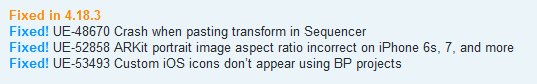
\includegraphics[width=0.55\textwidth]{images/Changelog.png}	
\end{wrapfigure}
De versie vertelt verder niets over wat er veranderd is aan de applicatie, hiervoor wordt een changelog aangemaakt.
Bij elke versie word een changelog aangemaakt waarin de veranderingen duidelijk worden omgeschreven, door middel van Git kan er precies worden weergegeven welke veranderingen zijn toegepast door naar de commits tussen de releases te kijken.
Een voorbeeld hiervan is de changelog van Unreal Engine, een populaire game engine.

\section{Versie-nummers \& pre-releases}
Bij de opbouw van het versie nummer is het niet toegestaan om een nummer te laten beginnen met 0 (bv. 1.01.0 is niet toegestaan). Een uitzondering hierop is de opbouw van het versie nummer wanneer de software nog in ontwikkeling is zoals beschreven in \cref{sec:major}.

Wanneer ervoor gekozen wordt om een pre-release versie van de software beschikbaar te stellen, kan dit tevens worden weergegeven in het versie nummer. Dit gebeurd door de versie van de pre-release door middel van een koppelteken te plaatsen achter het daadwerkelijke versie nummer van de software. Een aantal voorbeelden hiervan zijn: 1.0.0-alpha, 1.0.0-alpha.1, 1.0.0-0.3.7

Eventuele build metadata mag tevens worden weergegeven in het versie nummer. Dit wordt gebruikelijk direct na het patch nummer of de pre-release versie weergegeven met behulp van het koppelteken +.